%----------------------------------------------------------------------------------------
%	PACKAGES AND THEMES
%----------------------------------------------------------------------------------------
\documentclass[aspectratio=169,xcolor=dvipsnames, t]{beamer}
\usepackage{fontspec} % Allows using custom font. MUST be before loading the theme!
\usetheme{SimplePlusAIC}
\usepackage{hyperref}
\usepackage{graphicx} % Allows including images
\usepackage{booktabs} % Allows the use of \toprule, \midrule and  \bottomrule in tables
\usepackage{svg} %allows using svg figures
\usepackage{tikz}
\usepackage{makecell}
\usepackage{wrapfig}
\usepackage{algorithm}
\usepackage{algorithmic}
\usepackage[style=ieee]{biblatex}
\addbibresource{ref.bib}

% ADD YOUR PACKAGES BELOW

%----------------------------------------------------------------------------------------
%	TITLE PAGE CONFIGURATION
%----------------------------------------------------------------------------------------

\title[Parareal Algorithm]{Parareal Algorithm} 

\author[O. BOUHENNICHE \and N. ZAOUACHE]{Oussama BOUHENNICHE \and Narimane ZAOUACHE \\[5mm]{\small Supervisors: M. Christophe PRUD’HOMME}}

\institute[]{University of Strasbourg}

\date{\today} % Date, can be changed to a custom date
%----------------------------------------------------------------------------------------
%	PRESENTATION SLIDES
%----------------------------------------------------------------------------------------

\begin{document}

\maketitlepage

\begin{frame}[t]{Overview}
    \tableofcontents
\end{frame}

%------------------------------------------------
% Section divider frame
\makesection{Introduction}

%------------------------------------------------
% Bullets
\begin{frame}{Context}
    \begin{itemize}
        \item Solving time-dependent ordinary differential equations (ODEs) and partial differential equations (PDEs) numerically is crucial in computational fields.
        \item Traditional methods can be highly time-consuming, especially for long simulations or intricate systems.
    \end{itemize}
\begin{block}{}
    The Parareal algorithm \footfullcite{lions2001resolution} provides an efficient parallel solution to expedite the solving of ODEs and PDEs
\end{block}
\end{frame}

%------------------------------------------------
% Lists
\begin{frame}{Objectives}
    \begin{enumerate}
        \item Study lorenz system \footfullcite{lorenz1963deterministic} and Implement Lorenz Model, also study different ODEs solvers and its implementation.
        \item Explore the scipy.integrate \footfullcite{SciPy} package for ODEs solving and test it on lorenz system.
        \item Study the Parareal algorithm and implement it in sequential.
        \item study the parallelisation mechanism of the Parareal algorithm and implement it.
    \end{enumerate}
\end{frame}

%------------------------------------------------
% Section divider frame
\makesection{Background}

%------------------------------------------------
\begin{frame}{Lorenz system and ODEs solvers}
    \begin{columns}
\begin{column}{0.5\textwidth}
  \begin{center}
\large
\begin{cases}
    \displaystyle\frac{dx}{dt} = \sigma(y - x) \\
    \displaystyle\frac{dy}{dt} = x(\rho - z) - y \\
    \displaystyle\frac{dz}{dt} = xy - \beta z
\end{cases}
  \end{center}\\
   
\end{column}
\begin{column}{0.5\textwidth}  %%<--- here
    where:
\begin{itemize}
    \item $x$ is the rate of convective overturning,
    \item $y$ is the horizontal temperature variation,
    \item $z$ is the vertical temperature variation,
    \item $\sigma $ is the Prandtl number,
    \item $\rho $ is the Rayleigh number,
    \item $\beta $ is a geometrical factor.
\end{itemize}
\end{column}
\end{columns}
\end{frame}

\begin{frame}{Lorenz system and ODEs solvers}

    \begin{columns}
\begin{column}{0.5\textwidth}
   \begin{figure}[ht!]
    \centering
    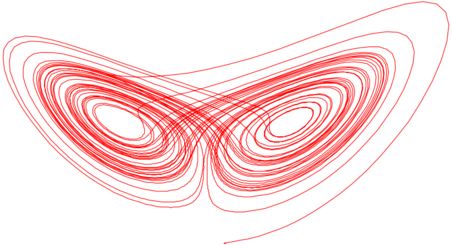
\includegraphics[width=0.8\textwidth]{figures/lorenz-attractor-112761.png}
    \caption{Lorenz attractor.}
    \label{fig:1}
\end{figure}
\end{column}
\begin{column}{0.5\textwidth}  %%<--- here
    \begin{center}
     \begin{figure}[ht!]
    \centering
    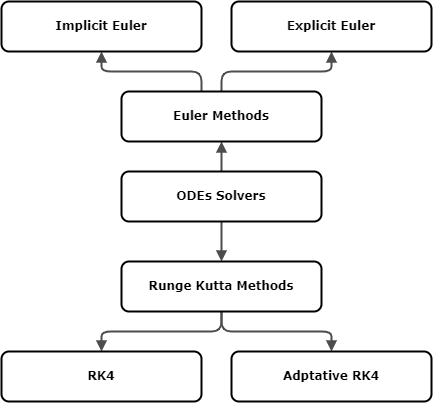
\includegraphics[width=0.7\textwidth]{figures/ode.png}
    \caption{ODEs solvers.}
    \label{fig:1}
\end{figure}
     \end{center}
\end{column}
\end{columns}
    
\end{frame}

\begin{frame}{Parareal Algorithm}
    \begin{itemize}
    \item \textbf{Core Idea}
    \begin{itemize}
        \item Accelerates time-dependent ODE/PDE solving using parallel computing.
        \item Decomposes the time domain into smaller intervals that can be processed simultaneously.
    \end{itemize}
    \item \textbf{How it Works}
    \begin{itemize}
        \item Combines coarse and fine propagators.
        \item Iteratively corrects the coarse solution with fine solution details.
    \end{itemize}
    \item \textbf{Stability}
    \begin{itemize}
        \item Stability depends on the choice of coarse and fine propagators.
        \item Typically stable for a wide range of problems.
    \end{itemize}
    \item \textbf{Parallelization}
    \begin{itemize}
        \item Distributes computation across multiple processors.
        \item Significantly reduces computation time for large-scale problems.
    \end{itemize}
\end{itemize}
\end{frame}

%------------------------------------------------
% Section divider frame
\makesection{Implementation and Results}

%------------------------------------------------
\begin{frame}{Sequential Parareal Algorithm}
    \begin{algorithm}[H]
\caption{Parareal Algorithm}
\begin{algorithmic}[1]
\STATE \textbf{Given:} Coarse function $G$, fine function $F$, number of time steps $N$, maximum number of iterations $K$, $\epsilon$ tolerance.
\STATE \textbf{Initialize:} \begin{itemize}
    \item  $U_0^0 = u_0$,
    \item $ U_{j+1}^0 = G(t_j,t_{j+1}, U_j^0) \;\;\;j = 0,1, \ldots, N-1$
\end{itemize}
\WHILE{$|U^k-U^{k-1}| > \epsilon $}
    \begin{itemize}
        \item  $ U_{j+1}^k = G(t_j,t_{j+1},U_j^k) + F(t_j,t_{j+1},U_j^{k-1}) -G(t_j,t_{j+1},U_j^{k-1})\;\;\;\;\;\;\;\;\;\;\newline j = 0,1, ... ,N-1$.
    \end{itemize}
\ENDWHILE
\STATE \textbf{Return:} $U^k$
\end{algorithmic}
\end{algorithm}
\end{frame}

\begin{frame}{Parallel Parareal Algorithm}
    \begin{algorithm}[H]
\caption{Parareal Algorithm (parallel version)} 
\begin{algorithmic}[1]
\STATE \textbf{Given:} Coarse function $G$, fine function $F$, number of time steps $N$, maximum number of iterations $K$, $\epsilon$ tolerance, number of process.
\STATE \textbf{Initialize: in sequential} \begin{itemize}
    \item  $U_0^0 = u_0; \;\;\;\; U_{j+1}^0 = G(t_j,t_{j+1}, U_j^0) \;\;\;j = 0,1, \ldots, N-1$
\end{itemize}
\WHILE{$|U^k-U^{k-1}| > \epsilon $}
    \begin{itemize}
        \item run the fine solver on each process and given a sub-interval of the time slices, in parallel: $F(t_j,t_{j+1}, U_j^{k-1}) \;\;\;\;\;\;\;\;\;\; j = 0,1, ... ,N-1$.
        \item  communicate fine solution and update u in sequetial and share it to all process: $ U_{j+1}^k = G(t_j,t_{j+1},U_j^k) + F(t_j,t_{j+1},U_j^{k-1}) -G(t_j,t_{j+1},U_j^{k-1})$.  
    \end{itemize}
\ENDWHILE
\STATE \textbf{Return:} $U^k$
\end{algorithmic}
\end{algorithm}
\end{frame}

\begin{frame}{Results}
    \begin{columns}
\begin{column}{0.5\textwidth}
   \begin{figure}[ht!]
    \centering
    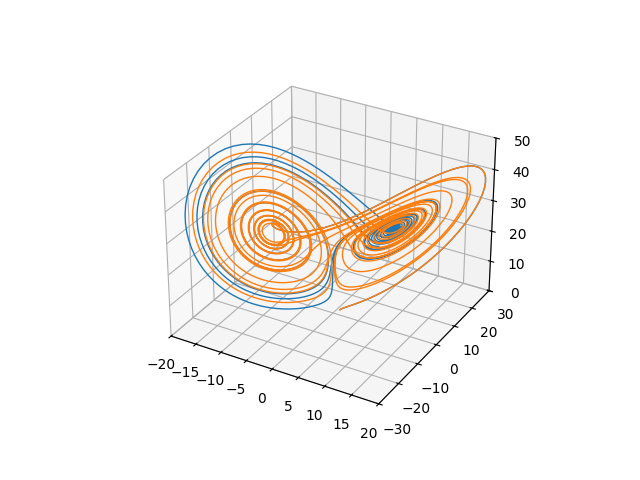
\includegraphics[width=0.9\textwidth]{figures/Figure_1.png}
    \caption{Lorenz chaotic phenomena}
    \label{fig:4}
\end{figure}
\end{column}
\begin{column}{0.5\textwidth}  %%<--- here
    \begin{center}
     \begin{figure}[H]
    \centering
    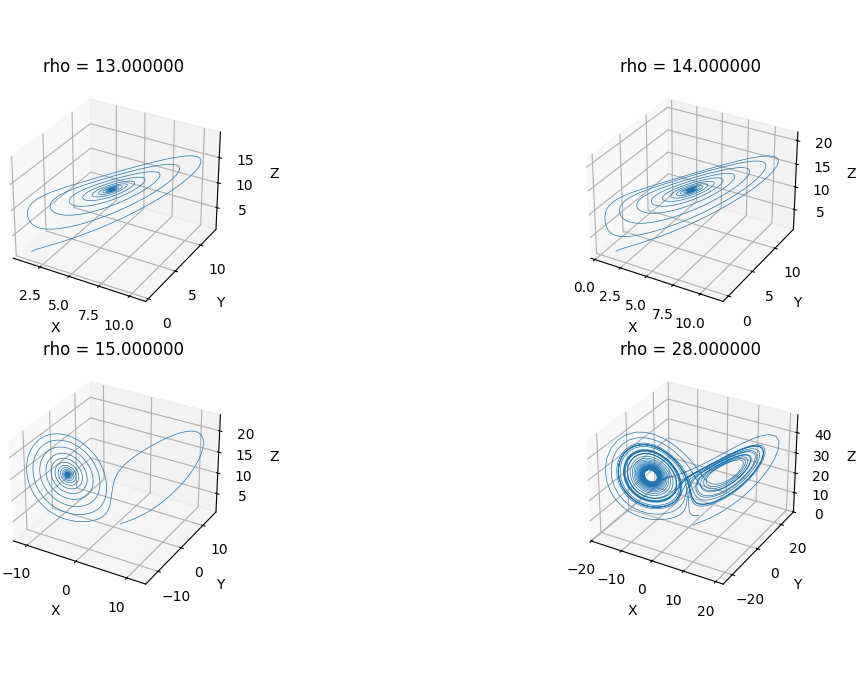
\includegraphics[width=.85\textwidth]{figures/lorenz_rho.png}
    \caption{Solutions of the Lorenz System Across Various $\rho$ Values}
    \label{fig:8}
\end{figure}
     \end{center}
\end{column}
\end{columns}
\end{frame}

\begin{frame}{Results}
    \begin{columns}
\begin{column}{0.5\textwidth}
   \begin{figure}[ht!]
    \centering
    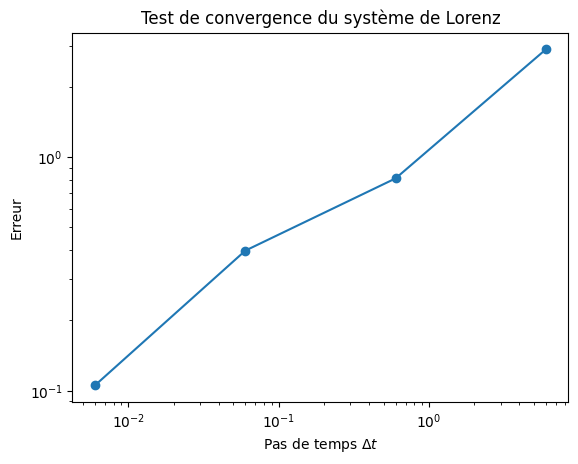
\includegraphics[width=0.78\textwidth]{figures/cv.png}
    \caption{Convergence check}
    \label{fig:5}
\end{figure}
\end{column}
\begin{column}{0.5\textwidth}  %%<--- here
    \begin{center}
     \begin{figure}[ht!]
    \centering
    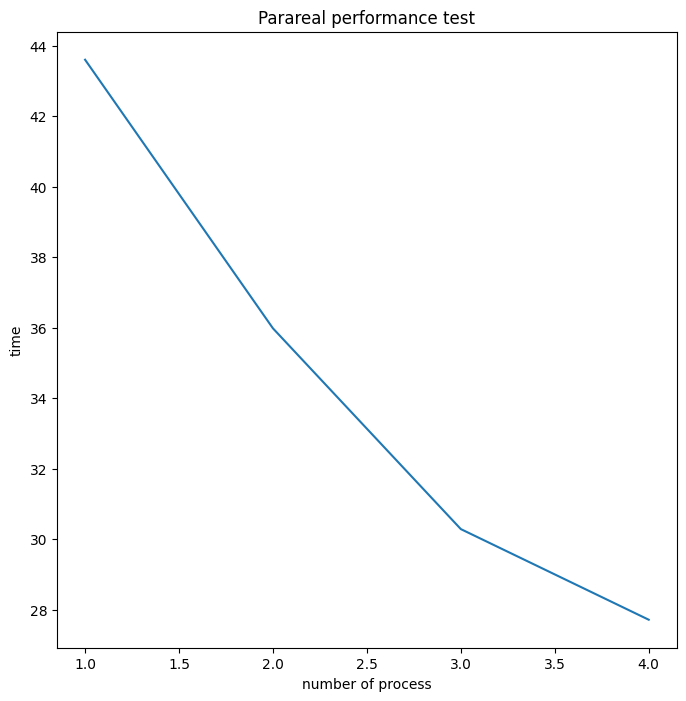
\includegraphics[width=0.64\textwidth]{figures/par.png}
    \caption{Parareal performance comparison by the number of process}
    \label{fig:6}
\end{figure}
     \end{center}
\end{column}
\end{columns}
\end{frame}

\begin{frame}{Results}
    \begin{figure}[ht!]
    \centering
    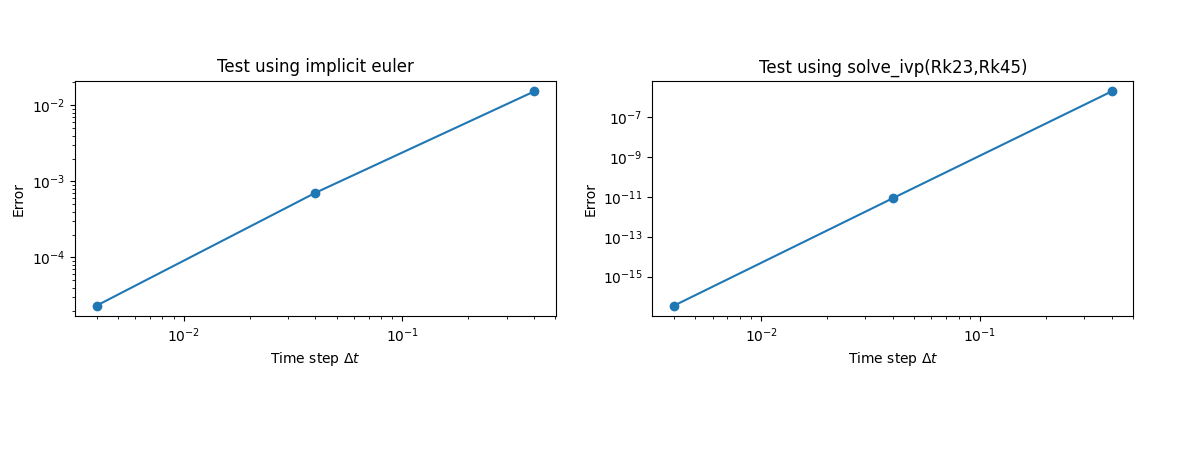
\includegraphics[width=1\textwidth]{figures/order_converge.png}
    \caption{Influence of Solver Choice on Parareal Convergence Order}
    \label{fig:9}
\end{figure}
\end{frame}

% Section divider frame
\makesection{Conclusion}
\begin{frame}{Conclusion}
\textbf{Diverse ODE Methods:}
\begin{itemize}
    \item Implemented and tested Euler, Runge-Kutta, and scipy.integrate methods on the Lorenz system.
\end{itemize}
\textbf{Parareal Algorithm:}
\begin{itemize}
    \item Implemented sequentially and in parallel.
    \item Significant reduction in computation time with increased processes.
    \item Demonstrated high potential for large-scale simulations.
\end{itemize}
\textbf{Future Prospects:}
\begin{itemize}
    \item Further exploration with Parareal for PDEs using frameworks like feel++.
\end{itemize}
\end{frame}

%------------------------------------------------
% Refenrenced
\begin{frame}[allowframebreaks]{References}
    %\nocite{*}
    \printbibliography
	
\end{frame}

%----------------------------------------------------------------------------------------
% Final PAGE
% Set the text that is showed on the final slide
\finalpagetext{Thank you for your attention}
%----------------------------------------------------------------------------------------
\makefinalpage
%----------------------------------------------------------------------------------------
\end{document}